\clearpage
\section{曲面积分：基本概念及定理}
\src{原书 §5.3，pp.270—273}
\entry{预备结论}{光滑曲面片及面积}{pp.270—271}
设光滑曲面片 $S$ 的参数为
\[
\rr=\rr(u,v)=x(u,v)\vct i+y(u,v)\vct j+z(u,v)\vct k,
\qquad (u,v)\in D,
\]
其中 $x,y,z$ 有连续偏导数，且 $\rr_u\times\rr_v\ne\vct0$。曲面面积为
\[
|S|=\iint_D|\rr_u\times\rr_v|\dd u\dd v.
\]
当曲面写为 $z=f(x,y)$ 时，
\begin{equation}
|S|=\iint_D\sqrt{1+f_x^2+f_y^2}\dd x\dd y.\tag{5.3.1}
\end{equation}

\entry{定义 5.3.1}{第一型曲面积分}{p.271}
设 $S$ 为有界光滑曲面，$f$ 定义于其上。将 $S$ 分为小片 $S_i$，面积记为 $\Delta S_i$，任取介点 $P_i=(\xi_i,\eta_i,\zeta_i)\in S_i$。若极限
\[
\lim_{\lambda\to0}\sum_i f(P_i)\Delta S_i
\]
存在且有限，并与介点选取无关（$\lambda$ 为小片的最大直径），则记为 $\iint_S f(x,y,z)\dd S$，称为第一型曲面积分。

\entry{定理 5.3.1}{第一型曲面积分的计算}{p.271}
设有界光滑曲面 $S$ 具有参数 $\rr(u,v)$，$D$ 为 $Ouv$ 平面内有界闭域，$f$ 在包含 $S$ 的区域内连续，则第一型曲面积分存在，且
\begin{equation}
\iint_S f\dd S=\iint_D f(x(u,v),y(u,v),z(u,v))|\rr_u\times\rr_v|\dd u\dd v,\tag{5.3.2}
\end{equation}
也可写为
\begin{equation}
\iint_S f\dd S=\iint_D f(x(u,v),y(u,v),z(u,v))\sqrt{EG-F^2}\dd u\dd v,\tag{5.3.3}
\end{equation}
其中 $E=|\rr_u|^2$、$G=|\rr_v|^2$、$F=\rr_u\cdot\rr_v$ 为 Gauss 系数。
特别地，若 $S:z=z(x,y)$，则
\[
\iint_S f\dd S=\iint_D f(x,y,z(x,y))\sqrt{1+z_x^2+z_y^2}\dd x\dd y.
\]

\entry{定义 5.3.2}{第二型曲面积分}{pp.271—272}
设 $S$ 为三维向量场 $\FF$ 中的定向光滑曲面，$\nn$ 为单位法向量。将曲面分为面积片，选取介点 $M_i$，若小片最大直径趋于零时，极限
\[
\sum_i\FF(M_i)\cdot\nn(M_i)\Delta S_i
\]
存在，且不依赖于取点，则称为第二型曲面积分，记为
\[
\iint_S\FF\cdot\dd\vct S=\iint_S\FF\cdot\nn\dd S,
\qquad\dd\vct S=\nn\dd S.
\]
这里 $\dd\vct S$ 为有向面积微元。设 $\FF=(P,Q,R)$，$\nn$ 与 $x,y,z$ 轴的夹角分别为 $\alpha,\beta,\gamma$，则
\[
\nn=(\cos\alpha,\cos\beta,\cos\gamma),\quad
\FF\cdot\nn\dd S=P\cos\alpha\dd S+Q\cos\beta\dd S+R\cos\gamma\dd S.
\]
令
\[
\dd y\wedge\dd z=\cos\alpha\dd S,\quad
\dd z\wedge\dd x=\cos\beta\dd S,\quad
\dd x\wedge\dd y=\cos\gamma\dd S,
\]
则
\[
\iint_S\FF\cdot\dd\vct S
=\iint_S[P\dd y\wedge\dd z+Q\dd z\wedge\dd x+R\dd x\wedge\dd y].
\]
记号 $\wedge$ 常略去。

\entry{定理 5.3.2}{第二型曲面积分的参数计算}{p.272}
设 $S$ 的参数为 $\rr=(x(u,v),y(u,v),z(u,v))$，定向为
$\nn=(\rr_u\times\rr_v)/|\rr_u\times\rr_v|$，则
\begin{align*}
\iint_S\FF\cdot\dd\vct S
&=\iint_D\FF\cdot(\rr_u\times\rr_v)\dd u\dd v\\
&=\iint_D\begin{vmatrix}P&Q&R\\x_u&y_u&z_u\\x_v&y_v&z_v\end{vmatrix}\dd u\dd v\\
&=\iint_D\left[P\frac{\partial(y,z)}{\partial(u,v)}+Q\frac{\partial(z,x)}{\partial(u,v)}+R\frac{\partial(x,y)}{\partial(u,v)}\right]\dd u\dd v.
\end{align*}

\entry{定理 5.3.3}{Gauss 公式}{p.272}
设 $V$ 由分片光滑双侧封闭曲面 $S$ 围成，$S$ 取向外方向，$P,Q,R$ 在 $V$ 上有连续一阶偏导数，则
\[
\oiint_{\partial V}P\dd y\dd z+Q\dd z\dd x+R\dd x\dd y
=\iiint_V(P_x+Q_y+R_z)\dd x\dd y\dd z.
\]

\entry{定理 5.3.4}{Stokes 公式}{pp.272—273}
设分片光滑曲面 $S$ 以封闭曲线 $L$ 为边界，$P,Q,R$ 在包含 $S$ 的空间区域内有连续偏导数，则
\begin{align*}
\oint_L P\dd x+Q\dd y+R\dd z
=\iint_S\bigl[&(R_y-Q_z)\dd y\dd z+(P_z-R_x)\dd z\dd x\\
&+(Q_x-P_y)\dd x\dd y\bigr].
\end{align*}
其中 $L$ 的取向与 $S$ 协调，即 $L$ 的方向与曲面法向成右手系。

\clearpage
\section{曲面积分：例题及原解}
\entry{例 5.3.1}{第一卦限球面上的第一型积分}{p.273}
设 $S$ 为第一卦限球面 $x^2+y^2+z^2=R^2$，$x,y,z\ge0$，求 $\iint_S(x^2+y^2)\dd S$。
\sol 由对称性，
\begin{align*}
I&=2\iint_Sx^2\dd S=\frac23\iint_S(x^2+y^2+z^2)\dd S\\
&=\frac{2R^4}{3}\int_0^{\pi/2}\dd\varphi\int_0^{\pi/2}\sin\theta\dd\theta
=\frac{\pi R^4}{3}.
\end{align*}

\entry{例 5.3.2}{柱面所截锥面上的积分}{p.273}
设 $S$ 为锥面 $z^2=k^2(x^2+y^2)$、$z\ge0$ 被柱面 $x^2+y^2=2ax$（$a>0$）所截得的曲面，求 $\iint_S(y^2z^2+z^2x^2+x^2y^2)\dd S$。
\sol 有 $\dd S=\sqrt{1+z_x^2+z_y^2}\dd x\dd y=\sqrt{1+k^2}\dd x\dd y$，投影域为 $D:x^2+y^2\le2ax$。故
\begin{align*}
I&=\sqrt{1+k^2}\iint_D[k^2(x^2+y^2)^2+x^2y^2]\dd x\dd y\\
&=2\sqrt{1+k^2}\int_0^{\pi/2}\dd\varphi\int_0^{2a\cos\varphi}r^5(k^2+\cos^2\varphi\sin^2\varphi)\dd r\\
&=\frac\pi{24}a^6(80k^2+7)\sqrt{1+k^2}.
\end{align*}

\entry{例 5.3.3}{柱侧面上的积分}{p.274}
设 $S$ 为柱面 $x^2+y^2=a^2$ 被 $z=0$、$z=h$（$h>0$）截下的柱面，求 $\iint_S(x^4+y^4)\dd S$。
\sol 取参数 $\rr=(a\cos\varphi,a\sin\varphi,z)$，$0\le\varphi\le2\pi$、$0\le z\le h$。则
\[
\rr_\varphi=(-a\sin\varphi,a\cos\varphi,0),\quad\rr_z=(0,0,1),\quad
|\rr_\varphi\times\rr_z|=a.
\]
由对称性，$\iint_Sx^4\dd S=\iint_Sy^4\dd S$，故
\begin{align*}
I&=2\iint_Sy^4\dd S=2\int_0^h\int_0^{2\pi}a^4\sin^4\varphi\cdot a\dd\varphi\dd z\\
&=8a^5\int_0^{\pi/2}\sin^4\varphi\dd\varphi\cdot\int_0^h\dd z
=\frac32\pi ha^5.
\end{align*}

\entry{例 5.3.4}{球体的平面截面}{pp.274—275}
设 $S(t)$ 为平面 $M(t):x+y+z=t$ 被球 $x^2+y^2+z^2=1$ 截下的部分，$F=1-(x^2+y^2+z^2)$。证明当 $|t|\le\sqrt3$ 时，
\[
\iint_{S(t)}F\dd S=\frac{\pi(3-t^2)^2}{18}.
\]
\prooftext 单位法向量为 $\nn=(1,1,1)/\sqrt3$，原点到平面的距离为 $|t|/\sqrt3$。当 $|t|>\sqrt3$ 时，平面不交球体 $B$；当 $|t|<\sqrt3$ 时，截面为圆盘，中心为 $(t/3,t/3,t/3)$，半径为 $r_0=\sqrt{1-t^2/3}$。
距圆心为 $r$ 的点满足
\[
(x-t/3)^2+(y-t/3)^2+(z-t/3)^2=r^2.
\]
结合 $x+y+z=t$，得 $x^2+y^2+z^2=t^2/3+r^2$。在该平面内取极坐标，$\dd S=r\dd r\dd\varphi$，$(r,\varphi)\in[0,r_0]\times[0,2\pi]$。于是
\begin{align*}
I&=\iint\left[1-\left(\frac{t^2}3+r^2\right)\right]r\dd r\dd\varphi
=2\pi\int_0^{r_0}(r_0^2-r^2)r\dd r\\
&=2\pi\left(\frac{r_0^4}2-\frac{r_0^4}4\right)
=\frac{\pi r_0^4}2=\frac{\pi(3-t^2)^2}{18}.
\end{align*}

\entry{例 5.3.5}{第一型曲面积分的正交变换}{pp.275—276}
设 $S$ 为光滑参数曲面 $\vct X=(x(u,v),y(u,v),z(u,v))$，$D\subset\mathbb R^2$，$f$ 为 $S$ 上连续函数，$\vct A=(a_{ij})$ 为三阶正交矩阵。令 $\widetilde{\vct X}=\vct A\vct X$，将 $S$ 变为 $\widetilde S:\widetilde{\vct X}=\widetilde{\vct X}(u,v)$。证明
\[
\iint_Sf(\vct X)\dd S=\iint_{\widetilde S}f(\vct A^{\mathsf T}\widetilde{\vct X})\dd\widetilde S.
\]
\prooftext 有 $\widetilde{\vct X}_u=\vct A\vct X_u$、$\widetilde{\vct X}_v=\vct A\vct X_v$，且
\begin{align*}
\widetilde E&=|\widetilde{\vct X}_u|^2=\widetilde{\vct X}_u^{\mathsf T}\widetilde{\vct X}_u
=\vct X_u^{\mathsf T}\vct A^{\mathsf T}\vct A\vct X_u
=\vct X_u^{\mathsf T}\vct X_u=|\vct X_u|^2=E,\\
\widetilde G&=G,\\
\widetilde F&=\widetilde{\vct X}_u^{\mathsf T}\widetilde{\vct X}_v
=\vct X_u^{\mathsf T}\vct A^{\mathsf T}\vct A\vct X_v
=\vct X_u^{\mathsf T}\vct X_v=F.
\end{align*}
故 $\widetilde E\widetilde G-\widetilde F^2=EG-F^2$。由第一型积分计算公式，
\begin{align*}
\iint_Sf(\vct X)\dd S
&=\iint_Df(\vct X(u,v))\sqrt{EG-F^2}\dd u\dd v\\
&=\iint_Df(\vct A^{\mathsf T}\widetilde{\vct X}(u,v))\sqrt{\widetilde E\widetilde G-\widetilde F^2}\dd u\dd v\\
&=\iint_{\widetilde S}f(\vct A^{\mathsf T}\widetilde{\vct X})\dd\widetilde S.
\end{align*}

\entry{例 5.3.6}{Poisson 公式}{p.276}
设 $S$ 为单位球面 $x^2+y^2+z^2=1$，$f(t)$ 在 $\mathbb R$ 上连续。证明
\[
\iint_Sf(ax+by+cz)\dd S=2\pi\int_{-1}^1f(kt)\dd t,\qquad k=\sqrt{a^2+b^2+c^2}.
\]
\prooftext $k=0$ 时 $a=b=c=0$，结论显然。设 $k>0$，令 $a_1=a/k$、$b_1=b/k$、$c_1=c/k$。单位向量 $(a_1,b_1,c_1)$ 可补成正交矩阵 $\vct A$，另两行为 $(a_2,b_2,c_2)$、$(a_3,b_3,c_3)$。
变换 $\widetilde{\vct X}=\vct A\vct X$ 使单位球面仍为单位球面 $\widetilde S$。由例 5.3.5，原积分等于 $\iint_{\widetilde S}f(k\widetilde x)\dd\widetilde S$。取
\[
\widetilde x=t,\quad\widetilde y=\sqrt{1-t^2}\sin\varphi,\quad
\widetilde z=\sqrt{1-t^2}\cos\varphi,\quad -1\le t\le1,\quad0\le\varphi\le2\pi.
\]
Gauss 系数为 $E=1/(1-t^2)$、$G=1-t^2$、$F=0$，故
\[
I=\int_{-1}^1\int_0^{2\pi}f(kt)\dd\varphi\dd t=2\pi\int_{-1}^1f(kt)\dd t.
\]
\ednote{末行迭代积分的微分次序按所列上下限规范为 $\dd\varphi\dd t$，不改变原解计算。}

\entry{例 5.3.7}{上半球面的第二型积分}{pp.276—277}
求 $I=\iint_Sx^2\dd y\dd z+y^2\dd z\dd x+z^2\dd x\dd y$，其中 $S$ 为上半球面 $x^2+y^2+z^2=a^2$、$z\ge0$，取上侧。
\sol 取 $x=a\sin\theta\cos\varphi$、$y=a\sin\theta\sin\varphi$、$z=a\cos\theta$，$0\le\theta\le\pi/2$、$0\le\varphi\le2\pi$，则 $\nn=(x,y,z)/a$。故
\begin{align*}
I&=\iint_S(x^2,y^2,z^2)\cdot\frac{(x,y,z)}a\dd S
=\frac1a\iint_S(x^3+y^3+z^3)\dd S\\
&=\frac1a\iint_Sz^3\dd S
=\frac1a\int_0^{2\pi}\int_0^{\pi/2}(a\cos\theta)^3a^2\sin\theta\dd\theta\dd\varphi\\
&=2\pi a^4\int_0^{\pi/2}\cos^3\theta\sin\theta\dd\theta=\frac{\pi a^4}2.
\end{align*}
\textbf{注 5.3.1}\quad 这里利用了奇函数 $x^3,y^3$ 在对称区间上的积分为零。

\entry{例 5.3.8}{上半椭球面的参数计算}{pp.277—278}
求 $I=\iint_Sx^3\dd y\dd z+y^3\dd z\dd x$，其中 $S$ 为上半椭球面 $x^2/a^2+y^2/b^2+z^2/c^2=1$、$z\ge0$，取上侧。
\sol 取参数 $x=a\sin\theta\cos\varphi$、$y=b\sin\theta\sin\varphi$、$z=c\cos\theta$，参数域 $D:0\le\varphi\le2\pi$、$0\le\theta\le\pi/2$。有
\[
\frac{\partial(y,z)}{\partial(\theta,\varphi)}=bc\sin^2\theta\cos\varphi,\quad
\frac{\partial(z,x)}{\partial(\theta,\varphi)}=ac\sin^2\theta\sin\varphi,\quad
\frac{\partial(x,y)}{\partial(\theta,\varphi)}=ab\cos\theta\sin\theta.
\]
$\rr_\theta\times\rr_\varphi$ 指向上侧。因此
\begin{align*}
\iint_Sx^3\dd y\dd z
&=\iint_Da^3\sin^3\theta\cos^3\varphi\cdot bc\sin^2\theta\cos\varphi\dd\theta\dd\varphi\\
&=a^3bc\int_0^{2\pi}\cos^4\varphi\dd\varphi\int_0^{\pi/2}\sin^5\theta\dd\theta
=\frac25\pi a^3bc.
\end{align*}
同理 $\iint_Sy^3\dd z\dd x=(2/5)\pi ab^3c$，合计
\[
I=\frac25\pi abc(a^2+b^2).
\]

\entry{例 5.3.9}{补面为四面体应用 Gauss 公式}{p.278}
求 $A=\iint_Sx\dd y\dd z+y\dd z\dd x+z\dd x\dd y$，其中
$S:\{x,y,z\ge0,\ x+y+z=1\}$，法向量与 $(1,1,1)$ 同向。
\sol 补上三个曲面
\[
\begin{aligned}
S_1&:\{x=0,\ y,z\ge0,\ y+z\le1\},\\
S_2&:\{y=0,\ x,z\ge0,\ x+z\le1\},\\
S_3&:\{z=0,\ x,y\ge0,\ x+y\le1\},
\end{aligned}
\]
组成四面体 $V$，$\partial V$ 取外法向。记 $\omega=x\dd y\dd z+y\dd z\dd x+z\dd x\dd y$。由 Gauss 公式，
\[
\oiint_{\partial V}\omega=\iiint_V3\dd x\dd y\dd z=3\cdot\frac13\cdot\frac12=\frac12.
\]
所以 $A=\frac12-(\iint_{S_1}\omega+\iint_{S_2}\omega+\iint_{S_3}\omega)$。三个补面上的积分均为零，故 $A=1/2$。
\begin{center}\begin{minipage}{\linewidth}\centering
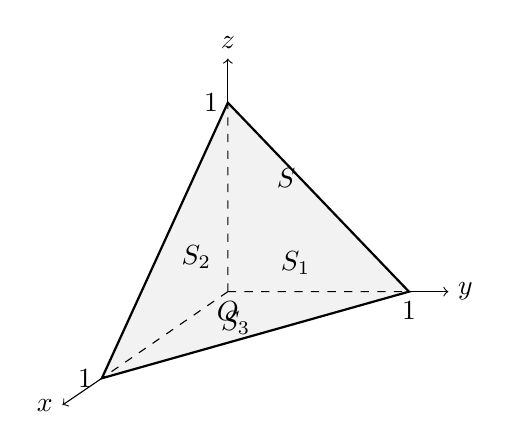
\begin{tikzpicture}[scale=2]
\coordinate(O)at(0,0);\coordinate(X)at(-.8,-.55);\coordinate(Y)at(1.15,0);\coordinate(Z)at(0,1.2);
\fill[gray!10](X)--(Y)--(Z)--cycle;
\draw[dashed](O)--(X)(O)--(Y)(O)--(Z);
\draw[thick](X)--(Y)--(Z)--cycle;
\draw[->](X)--(-1.05,-.72)node[left]{$x$};\draw[->](Y)--(1.4,0)node[right]{$y$};\draw[->](Z)--(0,1.48)node[above]{$z$};
\node[below]at(O){$O$};\node[above right]at(.25,.6){$S$};\node at(.43,.18){$S_1$};\node at(-.2,.22){$S_2$};\node at(.05,-.2){$S_3$};
\node[left]at(X){$1$};\node[below]at(Y){$1$};\node[left]at(Z){$1$};
\end{tikzpicture}\par{\small 图 5.3.1\quad 坐标面四面体与补面（重绘示意）}
\end{minipage}\end{center}
\textbf{注 5.3.2}\quad 当 $S$ 不封闭时，可补上若干光滑曲面，组成封闭曲面来应用 Gauss 公式，前提是补面的积分容易计算。

\entry{例 5.3.10}{平移球体上的 Gauss 公式}{pp.278—279}
求 $A=\iint_Sxy^2\dd y\dd z+yz^2\dd z\dd x+zx^2\dd x\dd y$，其中 $S$ 为球体 $V:\{x^2+y^2+z^2\le z\}$ 的外表面，方向朝外。
\sol 选取球体 $V$ 的参数
\[
x=r\cos\varphi\sin\theta,\quad y=r\sin\varphi\sin\theta,\quad z=\frac12+r\cos\theta,
\]
参数域为 $D:0\le r\le1/2$、$0\le\theta\le\pi$、$0\le\varphi\le2\pi$。由 Gauss 公式，
\begin{align*}
A&=\iiint_V(y^2+z^2+x^2)\dd V\\
&=\iiint_D\left[r^2\sin^2\theta+\frac14+r\cos\theta+r^2\cos^2\theta\right]r^2\sin\theta\dd r\dd\theta\dd\varphi\\
&=2\pi\int_0^\pi\int_0^{1/2}\left(r^2+\frac14+r\cos\theta\right)r^2\sin\theta\dd r\dd\theta\\
&=2\pi\left[\frac15\cdot\frac1{2^5}\cdot2+\frac14\cdot\frac13\cdot\frac1{2^3}\cdot2\right]=\frac\pi{15}.
\end{align*}

\entry{例 5.3.11}{反平方场的通量}{pp.279—280}
求 $I=\iint_S\cos(\rr,\nn)/r^2\dd S$，其中 $S$ 为光滑封闭曲面，原点不在 $S$ 上，$\rr=(x,y,z)$，$r=\sqrt{x^2+y^2+z^2}$，$\nn$ 为外单位法向量。
\sol 因 $\cos(\rr,\nn)=(\rr/r)\cdot\nn$，令
\[
\FF=(P,Q,R)=\left(\frac x{r^3},\frac y{r^3},\frac z{r^3}\right)=\frac{\rr}{r^3},
\]
则 $I=\iint_S\FF\cdot\nn\dd S$。有
\[
P_x=\frac{y^2+z^2-2x^2}{r^5}=\frac1{r^3}-\frac{3x^2}{r^5},\quad
Q_y=\frac1{r^3}-\frac{3y^2}{r^5},\quad R_z=\frac1{r^3}-\frac{3z^2}{r^5},
\]
故三者之和为零。

（1）若原点在 $S$ 外，则 $\FF$ 在其内域 $V$ 中连续可微，由 Gauss 公式，$I=\iiint_V\diver\FF\dd V=0$。

（2）若原点在 $S$ 内，则原点是 $\FF$ 的奇点。取以原点为中心、半径 $\varepsilon$ 的小球面 $S_\varepsilon\subset V$，定向向外。在两面间的夹域内场光滑，故
\[
\iint_{S-S_\varepsilon}\FF\cdot\nn\dd S=0.
\]
于是
\[
I=\iint_{S_\varepsilon}\FF\cdot\nn\dd S
=\iint_{S_\varepsilon}\frac{\rr}{r^3}\cdot\frac{\rr}r\dd S
=\iint_{S_\varepsilon}\frac1{\varepsilon^2}\dd S=4\pi.
\]

\entry{例 5.3.12}{梯度叉积的曲面积分（两解）}{p.280}
设 $S:\{x^2+y^2+z^2=1,\ z>0\}$ 取向上侧，
\[
f(x,y,z)=\frac{1+z}{1+x^2+y^2},\qquad g(x,y,z)=xy+yz+zx.
\]
求 $\iint_S\nabla f\times\nabla g\cdot\dd\vct S$。
\ednote{原书函数变量名写作 $f(x,y),g(x,y)$，但表达式含 $z$；此处补全三变量名。}
\par\textbf{原解·解法一}\quad 直接计算较繁，利用恒等式
\[
\diver(\nabla f\times\nabla g)
=\nabla\cdot(\nabla f\times\nabla g)
=\curl\nabla f\cdot\nabla g-\nabla f\cdot\curl\nabla g=0.
\]
补上底面 $S_1:\{x^2+y^2\le1,z=0\}$，定向与 $z$ 轴正向相反，即 $\nn_1=-\vct k$。由 Gauss 公式，
\[
\oiint_{S\cup S_1}\nabla f\times\nabla g\cdot\dd\vct S
=\iiint_\Omega\diver(\nabla f\times\nabla g)\dd V=0.
\]
所以
\[
\iint_S\nabla f\times\nabla g\cdot\dd\vct S
=-\iint_{S_1}\nabla f\times\nabla g\cdot\dd\vct S
=\iint_{S_1}\nabla f\times\nabla g\cdot\vct k\dd S.
\]
有
\[
\nabla f=\left(-\frac{2x(1+z)}{(1+x^2+y^2)^2},-\frac{2y(1+z)}{(1+x^2+y^2)^2},\frac1{1+x^2+y^2}\right),
\quad\nabla g=(y+z,z+x,x+y).
\]
在 $z=0$ 上，$(\nabla f\times\nabla g)\cdot\vct k=(-2x^2+2y^2)/(1+x^2+y^2)^2$。由对称性，底面积分为
\[
2\iint_{x^2+y^2\le1}\frac{y^2-x^2}{(1+x^2+y^2)^2}\dd x\dd y=0.
\]
\ednote{原书称底面法向与 $z$ 正向相反，却将 $\nn_1$ 印作 $\vct k$；此处明确为 $-\vct k$。}
\par\textbf{原解·解法二}\quad 因 $\nabla f\times\nabla g=\nabla\times(f\nabla g)$，由 Stokes 公式，
\[
\iint_S\nabla f\times\nabla g\cdot\dd\vct S
=\iint_S\nabla\times(f\nabla g)\cdot\dd\vct S
=\oint_{\partial S}f\nabla g\cdot\dd\rr.
\]
边圆 $\partial S:x^2+y^2=1,z=0$ 取协调正向，$f|_{\partial S}=1/2$，且 $\oint_{\partial S}\nabla g\cdot\dd\rr=0$，所以原积分为零。

\entry{例 5.3.13}{调和函数的球面平均值}{p.281}
设 $f$ 在闭球 $B(P_0,R)$ 上二阶连续，且 $\Delta f=f_{xx}+f_{yy}+f_{zz}=0$。证明
\[
f(P_0)=\frac1{4\pi r^2}\iint_Sf\dd S,
\]
其中 $P_0=(x_0,y_0,z_0)$，$S:(x-x_0)^2+(y-y_0)^2+(z-z_0)^2=r^2$，$0\le r\le R$。
\ednote{原书范围含 $r=0$，右端在该点按连续极限解释。}
\prooftext 令 $g(r)$ 为上式右端。取球面参数
\[
x=x_0+r\sin\theta\cos\varphi,\quad y=y_0+r\sin\theta\sin\varphi,\quad z=z_0+r\cos\theta,
\]
其中 $D:0\le\theta\le\pi$、$0\le\varphi\le2\pi$，记 $P$ 为该点。则
\[
g(r)=\frac1{4\pi}\iint_Df(P)\sin\theta\dd\theta\dd\varphi.
\]
记 $B_r=B(P_0,r)$，由 Gauss 公式，
\begin{align*}
g'(r)&=\frac1{4\pi}\iint_D\bigl[\sin\theta\cos\varphi f_x(P)+\sin\theta\sin\varphi f_y(P)\\
&\hspace{43mm}+\cos\theta f_z(P)\bigr]\sin\theta\dd\theta\dd\varphi\\
&=\frac1{4\pi r^2}\iint_S[f_x\dd y\dd z+f_y\dd z\dd x+f_z\dd x\dd y]\\
&=\frac1{4\pi r^2}\iiint_{B_r}\Delta f\dd V=0.
\end{align*}
故 $g$ 为常数，$g(r)=g(0)=f(P_0)$。

\entry{例 5.3.14}{三角形边界上的做功}{pp.281—282}
设 $S:\{x+y+z=1,\ x,y,z\ge0\}$，法向量与 $(1,1,1)$ 同向，$\FF=(y^2,z^2,x^2)$。求绕 $S$ 正向边界 $\partial S$ 一周所做的功。
\sol $\nn=(1,1,1)/\sqrt3$。由 Stokes 公式，
\begin{align*}
W&=\oint_{\partial S}\FF\cdot\dd\rr=\iint_S\curl\FF\cdot\nn\dd S\\
&=\iint_S(-2z,-2x,-2y)\cdot\nn\dd S
=-\frac2{\sqrt3}\iint_S(x+y+z)\dd S\\
&=-\frac2{\sqrt3}\cdot\frac{\sqrt3}{2}=-1.
\end{align*}
\begin{center}\begin{minipage}{\linewidth}\centering
\begin{tikzpicture}[scale=2,midarrow/.style={postaction={decorate},decoration={markings,mark=at position .55 with {\arrow{Stealth}}}}]
\coordinate(O)at(0,0);\coordinate(X)at(-.8,-.55);\coordinate(Y)at(1.15,0);\coordinate(Z)at(0,1.2);
\fill[gray!12](X)--(Y)--(Z)--cycle;
\draw[dashed](O)--(X)(O)--(Y)(O)--(Z);
\draw[thick,midarrow](X)--(Y);\draw[thick,midarrow](Y)--(Z);\draw[thick,midarrow](Z)--(X);
\draw[->](X)--(-1.05,-.72)node[left]{$x$};\draw[->](Y)--(1.4,0)node[right]{$y$};\draw[->](Z)--(0,1.48)node[above]{$z$};
\draw[->,thick,navy](.13,.22)--(.45,.85)node[right]{$\nn$};\node at(-.2,.35){$S$};\node[below]at(O){$O$};
\end{tikzpicture}\par{\small 图 5.3.2\quad 三角面、正向边界与法向（重绘）}
\end{minipage}\end{center}

\entry{例 5.3.15}{椭圆抛物面交线的环量}{p.282}
设 $L$ 为椭圆抛物面 $z=3x^2+4y^2$ 和椭圆柱面 $4x^2+y^2=4y$ 的交线，从 $z$ 轴正向看为顺时针。求 $\FF=(y(z+1),xz,xy-z)$ 沿 $L$ 的环量。
\sol 取 $D:4x^2+y^2\le4y$ 为 $Oxy$ 平面内区域，$S:z=3x^2+4y^2$、$(x,y)\in D$，方向朝下。由 Stokes 公式，
\[
\oint_L\FF\cdot\dd\rr=\iint_S\curl\FF\cdot\dd\vct S
=-\iint_S\dd x\dd y=\iint_D\dd x\dd y=2\pi.
\]
\begin{center}\begin{minipage}{\linewidth}\centering
\begin{tikzpicture}[x={(-.65cm,-.3cm)},y={(.7cm,-.25cm)},z={(0cm,.055cm)},scale=1.05]
\foreach \q in {-.9,-.45,0,.45,.9}{\draw[gray!45,thin]plot[domain=0:4,samples=24,variable=\t]({\q},{\t},{3*\q*\q+4*\t*\t});}
\foreach \q in {.4,1.2,2,2.8,3.6}{\draw[gray!45,thin]plot[domain=-1.1:1.1,samples=18,variable=\t]({\t},{\q},{3*\t*\t+4*\q*\q});}
\draw[dashed]plot[domain=0:360,samples=65,variable=\t]({cos(\t)},{2+2*sin(\t)},0);
\foreach \q in {0,90,180}{\draw[gray!55,dashed]({cos(\q)},{2+2*sin(\q)},0)--({cos(\q)},{2+2*sin(\q)},65);}
\draw[navy,thick]plot[domain=0:360,samples=90,variable=\t]({cos(\t)},{2+2*sin(\t)},{3*cos(\t)*cos(\t)+4*(2+2*sin(\t))^2});
\draw[->](0,0,0)--(1.7,0,0)node[left]{$x$};\draw[->](0,0,0)--(0,4.7,0)node[right]{$y$};\draw[->](0,0,0)--(0,0,75)node[above]{$z$};
\draw[->,thick](0,2,16)--(0,2,3)node[right]{\small 下侧};\node[right]at(0,4,64){$L$};\node[below]at(0,2,0){$D$};
\end{tikzpicture}\par{\small 图 5.3.3\quad 抛物面、柱面交线及下侧（重绘示意，非等比例）}
\end{minipage}\end{center}

\entry{例 5.3.16}{球面与柱面交线的 Stokes 计算}{pp.282—283}
求
\[
I=\oint_L(y^2+z^2)\dd x+(z^2+x^2)\dd y+(x^2+y^2)\dd z,
\]
其中 $L:\{x^2+y^2+z^2=2ax,\ x^2+y^2=2bx,\ z\ge0\}$，$0<b<a$；从 $x$ 轴正向看为逆时针。
\sol 取 $S$ 为 $L$ 在半球面 $x^2+y^2+z^2=2ax$、$z\ge0$ 内围出的面。从 $x$ 轴正向看为逆时针，故 $S$ 的方向朝下，指向球心，
\[
\nn=-\frac{(x-a,y,z)}a.
\]
由 Stokes 公式，
\begin{align*}
I&=2\iint_S(y-z,z-x,x-y)\cdot\nn\dd S\\
&=-2\iint_S(z-y)\dd S=-2\iint_Sz\dd S,
\end{align*}
其中关于 $y$ 的对称性使 $y$ 项积分为零。球面方程给出
\[
z=\sqrt{a^2-(x-a)^2-y^2},\qquad
\dd S=\sqrt{1+z_x^2+z_y^2}\dd x\dd y
=\frac a{\sqrt{a^2-(x-a)^2-y^2}}\dd x\dd y=\frac az\dd x\dd y.
\]
于是
\[
I=-2a\iint_D\dd x\dd y=-2a\pi b^2=-2\pi ab^2,
\qquad D:(x-b)^2+y^2\le b^2.
\]
\ednote{原书此处球面根号中 $y^2$ 前误作正号，面积元分母沿用该误号；此处两处均依球面方程校正为负号。}
\begin{center}\begin{minipage}{\linewidth}\centering
\begin{tikzpicture}[scale=.9]
\begin{scope}
\draw[gray](1.5,1.4)circle(1.4);\draw[gray,dashed](1.5,1.4)ellipse(1.4 and .32);
\draw[dashed](.9,.05)ellipse(.65 and .22);\draw[gray!65](.25,.05)--(.25,2.45)(1.55,.05)--(1.55,2.45);\draw[gray,dashed](.9,2.45)ellipse(.65 and .22);
\draw[navy,thick]plot[smooth]coordinates{(.25,1.4)(.4,2.05)(.85,2.58)(1.35,2.2)(1.55,1.5)(1.15,1.2)(.65,1.12)(.25,1.4)};
\fill(1.5,1.4)circle(1.3pt)node[right]{$(a,0,0)$};\node[left]at(.3,2.15){$L$};\node at(1,-.5){\small 球面与柱面示意};
\end{scope}
\begin{scope}[shift={(5,1.3)}]
\fill[gray!12](.9,0)circle(.9);\draw[thick](.9,0)circle(.9);
\draw[->](-.3,0)--(2.25,0)node[right]{$x$};\draw[->](0,-1.2)--(0,1.3)node[above]{$y$};
\fill(.9,0)circle(1.2pt);\node[below]at(.9,0){$b$};\node[below left]at(0,0){$O$};\node at(.9,.45){$D$};\node at(.9,-1.8){\small 投影圆盘};
\end{scope}
\end{tikzpicture}\par{\small 图 5.3.4\quad 球面、柱面及投影（重绘示意，交线方向见题设）}
\end{minipage}\end{center}

\entry{例 5.3.17}{圆柱斜截椭圆的环量}{p.283}
求
\[
I=\oint_L(y-z)\dd x+(z-x)\dd y+(x-y)\dd z,
\]
其中 $L$ 为柱面 $\Sigma_2:x^2+y^2=a^2$ 与平面 $\pi_1:x/a+z/h=1$（$a,h>0$）的交线，从 $x$ 轴正向看为逆时针。
\sol 取 $S$ 为平面 $\pi_1$ 被柱面截下的部分，$L=\partial S$。其投影为
\[
D_{xy}:x^2+y^2\le a^2,\qquad
D_{yz}:\frac{y^2}{a^2}+\frac{(z-h)^2}{h^2}\le1,
\]
在 $Oxz$ 平面上的投影为直线段。由 Stokes 公式，
\begin{align*}
I&=-2\iint_S[\dd y\dd z+\dd z\dd x+\dd x\dd y]\\
&=-2\iint_{D_{yz}}\dd y\dd z-2\iint_{D_{xy}}\dd x\dd y\\
&=-2\pi ah-2\pi a^2=-2\pi(a+h)a.
\end{align*}
\begin{center}\begin{minipage}{\linewidth}\centering
\begin{tikzpicture}[x={(.9cm,-.3cm)},y={(.55cm,.25cm)},z={(0cm,.9cm)},scale=1.1]
\draw[gray]plot[domain=0:360,samples=70,variable=\t]({cos(\t)},{sin(\t)},0);
\draw[gray]plot[domain=0:360,samples=70,variable=\t]({cos(\t)},{sin(\t)},2.5);
\draw[gray](-1,0,0)--(-1,0,2.5)(1,0,0)--(1,0,2.5);
\fill[gray!12]plot[domain=0:360,samples=70,variable=\t]({cos(\t)},{sin(\t)},{1.2*(1-cos(\t))})--cycle;
\draw[thick,navy,postaction={decorate},decoration={markings,mark=at position .2 with {\arrow{Stealth}},mark=at position .7 with {\arrow{Stealth}}}]plot[domain=0:360,samples=90,variable=\t]({cos(\t)},{sin(\t)},{1.2*(1-cos(\t))});
\draw[->](0,0,0)--(1.7,0,0)node[right]{$x$};\draw[->](0,0,0)--(0,1.7,0)node[right]{$y$};\draw[->](0,0,0)--(0,0,3)node[above]{$z$};
\draw[->,thick](0,0,1.2)--(.65,0,1.8)node[right]{$\nn$};\node[left]at(-1,0,2.4){$L$};\node[below left]at(0,0,0){$O$};
\end{tikzpicture}\par{\small 图 5.3.5\quad 圆柱与斜截椭圆的协调取向（重绘）}
\end{minipage}\end{center}

\entry{例 5.3.18}{球面大圆上的线性场积分}{pp.283—284（上半页）}
设 $a,b,c$ 不全为零，$L$ 为球面 $S:x^2+y^2+z^2=R^2$（$R>0$）与平面 $\Sigma:ax+by+cz=0$ 的交线，$L$ 的正向与平面法向量 $(a,b,c)$ 成右手系。求
\[
I=\oint_L(bz+c)\dd x+(cx+a)\dd y+(ay+b)\dd z.
\]
\sol 球体与平面截得大圆盘 $D$，其单位法向量为
\[
\nn=\frac{(a,b,c)}{\sqrt{a^2+b^2+c^2}},
\]
$L$ 为 $D$ 的边界。由 Stokes 公式，
\begin{align*}
I&=\iint_D\curl(bz+c,cx+a,ay+b)\cdot\nn\dd S\\
&=\iint_D(a,b,c)\cdot\nn\dd S
=\sqrt{a^2+b^2+c^2}\iint_D\dd S\\
&=\sqrt{a^2+b^2+c^2}\,\pi R^2.
\end{align*}
